\chapter{Evaluierung}

\section{Meinungen}

\begin{quote}
``Joa, ganz gut'' \\
``Die Karten kann man nicht so gut erkennen'' \\
``Aber sonst ist es so gut'' \\
``Die Navigation ist ziemlich einfach'' \\
``Die Hilfen [bei Schach] finde ich ganz gut'' \\
``Ich finde es gut, dass es mehrere Spiele zur Auswahl gibt''
\end{quote}
--- Lena, 14 Jahre, Schachanfängerin
\begin{quote}
``Die App ist einfach zu bedienen und macht Spaß'' \\
``Am Anfang ist die Startseite etwas leer'' 
\end{quote}
--- Tamara, 20 Jahre, 1. Semester Medieninformatik

\section{Wie gewinnt man ein Schafkopfspiel?}
\sectionauthor{\philipp}
Startet man unsere Spielesammlung und wählt Kartenspiele aus, dann hat man die Auswahl zwischen drei verschiedenen Spielen: Bauernkrieg, Mau Mau und Offiziersschafkopf.
\begin{figure}[h]
	\centering
	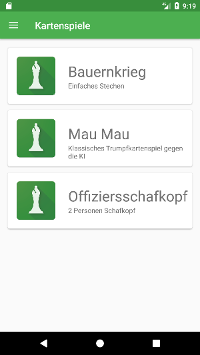
\includegraphics{resources/kartenscreens/auswahl}
	\caption{Auswahl der Spiele}
\end{figure}
Startet man eines dieser Spiele, wird man auf ein weiteres Menu weitergeleitet, auf welchem man jeweils nochmal die Regeln lesen kann wenn man auf das \emph{i} klickt.
\begin{figure}[h]
	\centering
	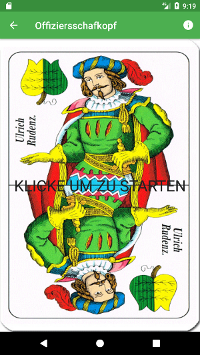
\includegraphics{resources/kartenscreens/menu}
	\caption{Spielmenu}
\end{figure}
Um Schafkopf spielen zu können, muss man jedoch die Regeln für das Bekennen und Stechen kennen. Klickt man auf das Bild in der Mitte, dann startet das Spiel und  das Feld wird aufgebaut. 
\begin{figure}[h]
	\centering
	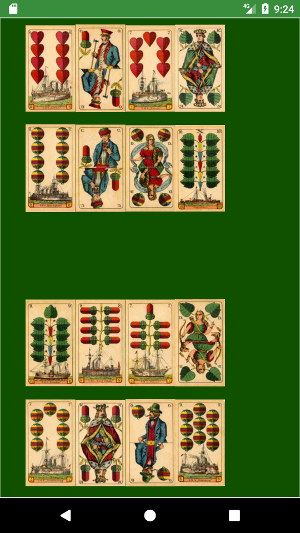
\includegraphics{resources/kartenscreens/board}
	\caption{Spielfeld Schafkopf}
\end{figure}
Der Spieler am unteren Bildschirmrand ist zuerst an der Reihe und darf eine Karte durch langes Drücken auswählen, Spieler zwei muss nun nach den Regeln bekennen, denn aufgrund eines Personalausfalls im Entwicklungsteam musste ich ein Feature streichen welches den Spieler dazu zwingt die richtige Karte zu legen. Hat er dies getan, wird der Stich automatisch ausgewertet und auf den richtigen Ablagestapel gezogen. Derjenige, der den Stich eingefahren hat ist nun an der Reihe mit Ausspielen. Das geht solange, bis kein Spieler mehr Karten hat. Sind alle Karten gespielt, werden die Punkte ausgewertet und der Gewinner/Verlierer samt Punkten angezeigt.
\begin{figure}[h]
	\centering
	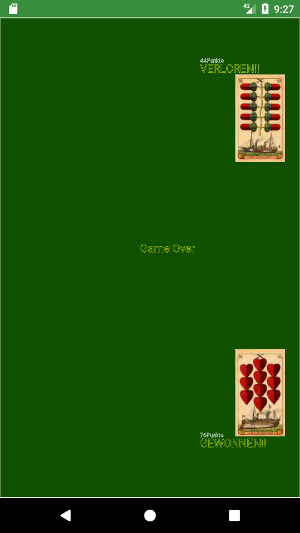
\includegraphics{resources/kartenscreens/gameover}
	\caption{Gameover Punkteanzeige}
\end{figure}
Mit einem klick auf den zurück-Knopf des Handy gelangt man wieder auf das Menu und kann das Spiel neustarten oder ein anderes auswählen.